\documentclass[problem]{mcs}

\begin{pcomments}
  \pcomment{FP_probable_isomorphism}
  \pcomment{from S09.final}
\end{pcomments}

\pkeywords{
 probability
 isomomorphism
 vertex}

%%%%%%%%%%%%%%%%%%%%%%%%%%%%%%%%%%%%%%%%%%%%%%%%%%%%%%%%%%%%%%%%%%%%%
% Problem starts here
%%%%%%%%%%%%%%%%%%%%%%%%%%%%%%%%%%%%%%%%%%%%%%%%%%%%%%%%%%%%%%%%%%%%%

\begin{problem} Let $G$ be the following graph:
 
 \begin{center}
 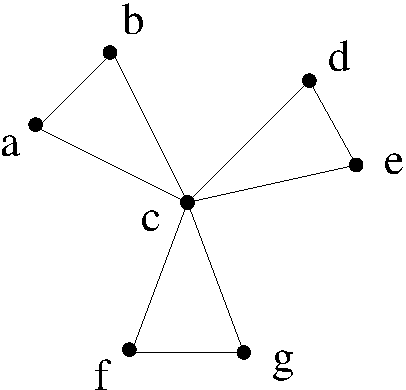
\includegraphics[width=1.5in]{simple-automorphims}
%{S09_final7.pdf}
 \end{center} 

 \bparts
 
 \ppart How many isomorphisms are there from $G$ to itself?  Show 
   your work or we can't award any partial credit. 

\exambox{2in}{0.75in}{-0.35in}
\examspace[2in]

\begin{solution}
$2^3 \cdot 3! = 48$
\end{solution}

 \ppart Let $f : \vertices{G} \to \vertices{G}$ be a randomly chosen
 bijection from $\vertices{G}$ to itself. What is the probability that
 $f$ is an isomorphism given $f(a) = a$.

\exambox{2in}{0.75in}{-0.35in}
\examspace[2in]

\begin{solution}
\[
\frac{2! \cdot 2^2}{6!}=\frac{1}{90}
\]
\end{solution}

 \eparts
\end{problem}

\endinput
